\documentclass{article}
\usepackage[utf8]{inputenc}
\usepackage{amsmath}
\usepackage{amssymb}
\usepackage{graphicx}
\usepackage{mathabx}

\begin{document}
\section*{Multiplication and division of polynomials based on DFT}

We call a \textbf{polynomial} in $x$ of \textbf{degree} $N \in\mathbb{N}$ a function $p : \mathbb{K} \to \mathbb{K}$ of the form 
\begin{equation*}
    p\left(x\right) = \sum_{i=0}^{N}\gamma_{i}x^{j} \text{ with \textbf{coefficients }} \gamma_{i} \in \mathbb{K}
\end{equation*}
also called \textbf{monomial representation}. The polynomials of degree $N$ for a vector space $\mathcal{P}_{N}$ of dimension $N+1$ (under pointwise additon and multiplication). We can represent every polynomial of degree $N$ by
\begin{equation*}
    \mathbf{c} := \left[\gamma_{0}, \dots, \gamma_{N}\right] \in \mathbb{K}^{N+1}
\end{equation*}
this gives an isomorphism from the vector space $\mathcal{P}_{n}$ to $\mathbb{K}^{N+1}$. We use this to represent polynomials in $\mathcal{P}_{N}$ using an object of type \verb|Eigen::VectorXd| containing their corresponding coefficient vectors. Let two large numbers $m,n \gg 1$ and two polynomials of degrees $m-1$ and $n-1$, respectively, in monomial representation
\begin{equation*}
    u\left(x\right) = \sum_{j=0}^{m-1}\alpha_{j}x^{j}\,,\quad v\left(x\right) = \sum_{j=0}^{n-1}\beta_{j}x^{j}\, \quad \alpha_{j},\beta_{j}\in \mathbb{C}
\end{equation*}
\subsection*{4-3.a}
We are tasked with using the basic polynomial multiplication to implement a method that multiplies two vectors given as \verb|Eigen::VectorXd| parameters and return the result. Let us look at the structure of the multiplication of the two multiplications.
\begin{equation*}
    u\left(x\right)\cdot v\left(x\right) = \sum_{j=0}^{m-1}\alpha_{j}x^{j}\cdot \sum_{j=0}^{n-1}\beta_{j}x^{j}
\end{equation*}
Here the structure is not as visible, let us thus start with a small example.
\begin{align*}
    u \cdot v &= 
    \left(\alpha_{0} + \alpha_{1}x^{1} + \alpha_{2}x^{2}\right) \cdot \left(\beta_{0} + \beta_{1}x^{1} + \beta_{2}x^{2}\right) \\&= \alpha_{0}\beta_{0} + \alpha_{0}\beta_{1}x^{1} + \alpha_{0}\beta_{2}x^{2} + \alpha_{1}\beta_{0}x^{1} + \alpha_{1}\beta_{1}x^{2} + \alpha_{1}\beta_{2}x^{3} + \alpha_{2}\beta_{0}x^{2} + \alpha_{2}\beta_{1}x^{3} + \alpha_{2}\beta_{2}x^{4} \\
    &= \alpha_{0}\beta_{0} + \left(\alpha_{0}\beta_{1} + \alpha_{1}\beta_{0}\right)x^{1} + \left(\alpha_{0}\beta_{2} + \alpha_{1}\beta_{1} + \alpha_{2}\beta_{0}\right)x^{2} + \left(\alpha_{1}\beta_{2} + \alpha_{2}\beta_{1}x^{3}\right) + \alpha_{2}\beta_{2}x^{4} \\
    &= \sum_{i=0}^{4}\sum_{a + b = i}\alpha_{a}\beta_{b}x^{i}
\end{align*}
This formula we can use to directly derive the general form by seeing that the resulting polynomial will have degree of the multiplied polynomials degrees summed together.
\begin{equation}
     u\left(x\right)\cdot v\left(x\right) = \sum_{i=0}^{m + n - 2}\sum_{a+b=i}\alpha_{a}\beta_{b}x^{i}
\end{equation} 

\pagebreak

\noindent We now have to implement the following sum.
\begin{equation*} \sum_{a+b=i}\alpha_{a}\beta_{b}x^{i}
\end{equation*}
This can be achieved by seeing that we can also write this as 
\begin{equation*}
    \sum_{a+b=i}\alpha_{a}\beta_{b}x^{i} = \sum_{a = \text{max}\left\{ 0,i -\left(n-1\right)\right\}}^{\text{min}\left\{i, \left(m-1\right)\right\}}\alpha_{a}\beta_{i - a}x^{i}
\end{equation*}
To understand what happens here one must look at the pattern of the sums and see how their start and end index of the $\alpha$ coefficients are dependent on $j$ and the degree of the polynomials. This gives us the following code.
\begin{figure}[!hbt]
    \centering
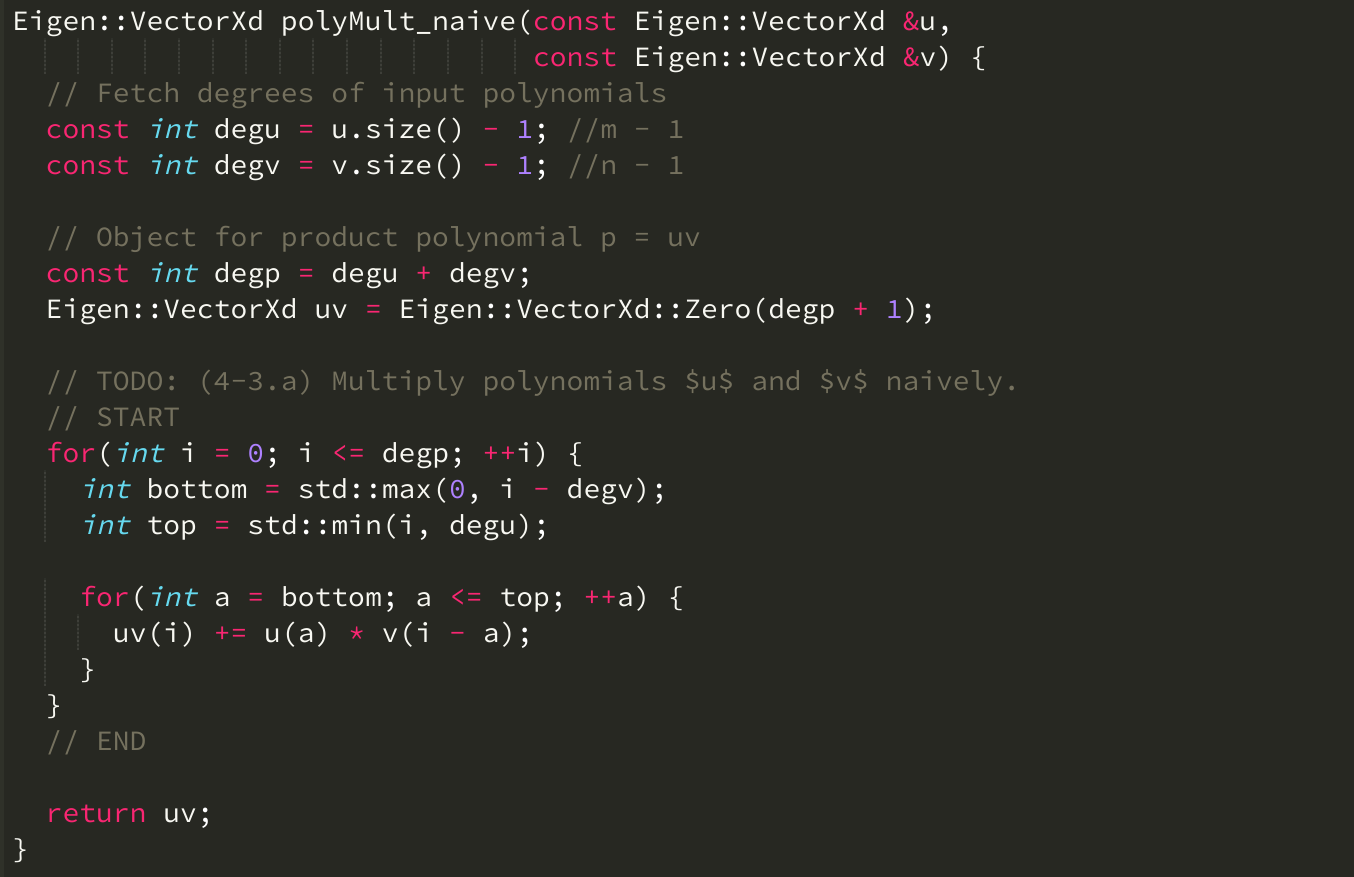
\includegraphics[width=1.0\linewidth]{4-3.a.png}
\end{figure}
\subsection*{4-3.b}
We are now tasked with writing a fast implementation using the DFT functionality of Eigen. We can see that when removing the terms $x^{i}$ the sum does resemble a discrete convolution. We have
\begin{equation*}
    \left(\mathbf{u}*\mathbf{v}\right)_{i} = \sum_{a=0}^{m-1}u_{a}v_{i - a}
\end{equation*}
where we use the convention that $v_{j} = 0$ for $j < 0$ or $j \geq n$. We can implement this convention by zero padding both input vectors to assure that this is the case. 

\pagebreak
\noindent To use DFT we need to apply the convolution theorem.
\begin{figure}[!hbt]
    \centering
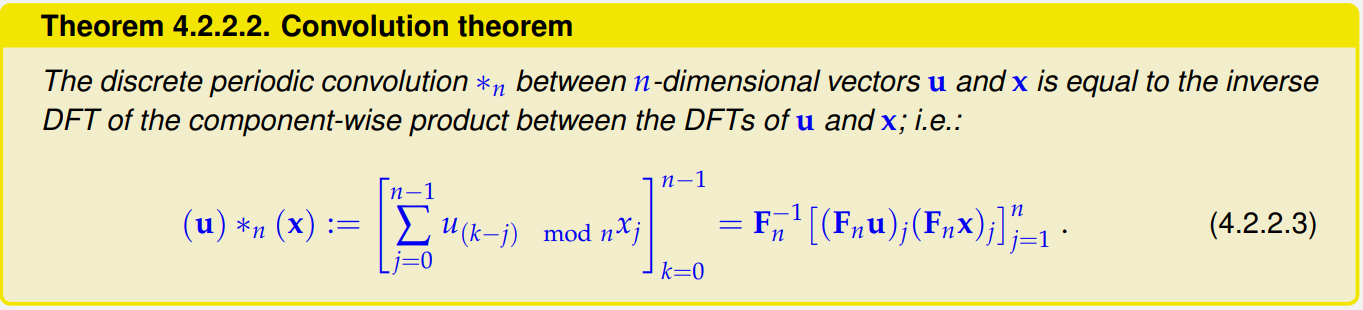
\includegraphics[width=1.0\linewidth]{ConvolutionTheorem.png}
\end{figure}

\noindent Just below this theorem we also find the following code segment which we will use as guide in our implementation. We need to use complex vectors as the FFT library requires them.

\begin{figure}[!hbt]
    \centering
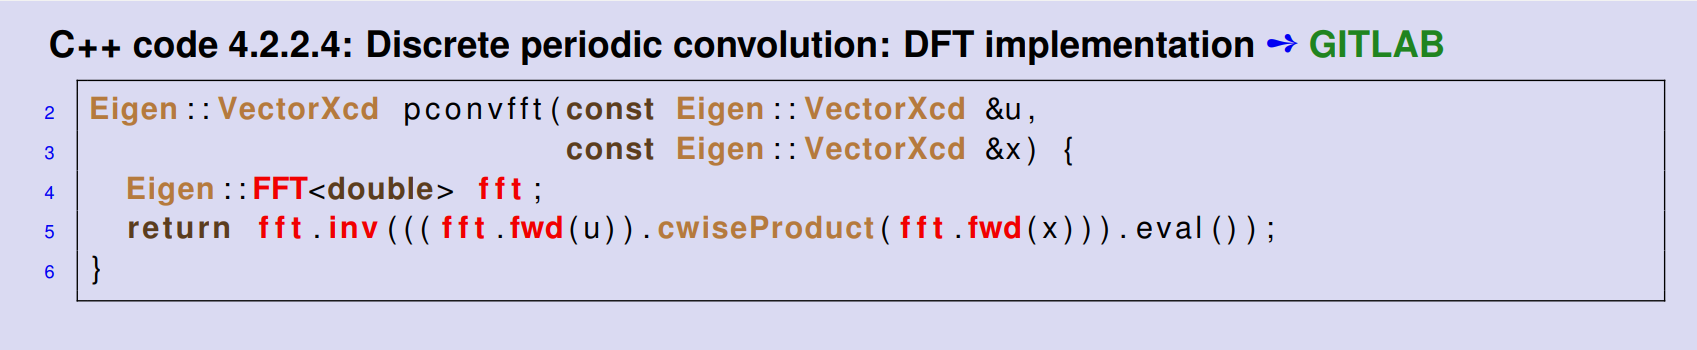
\includegraphics[width=1.0\linewidth]{DiscreteConvolutionWithFFT.png}
\end{figure}

\noindent This gives us the following code (remember to include \verb|<unsupported/Eigen/FFT>|).

\begin{figure}[!hbt]
    \centering
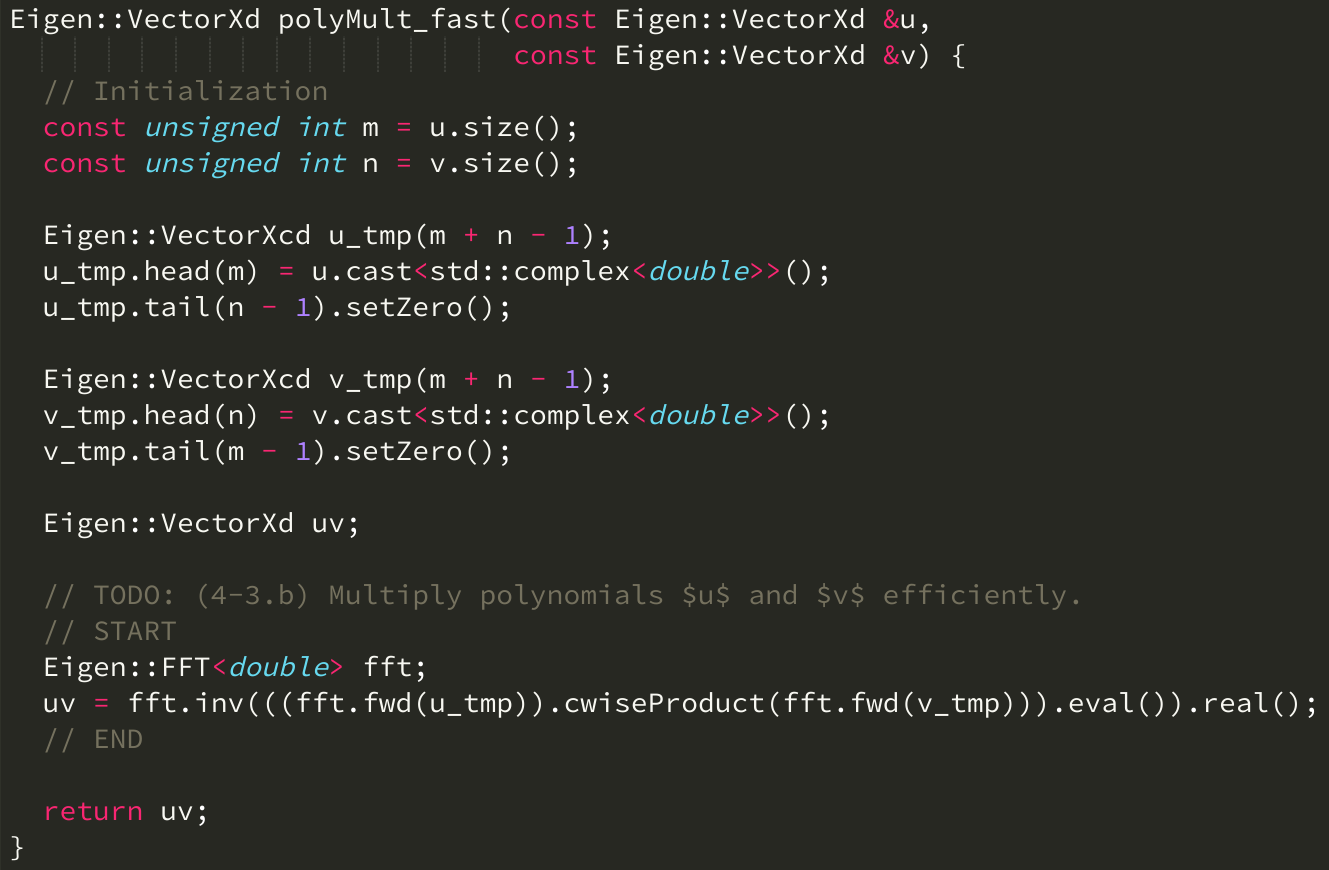
\includegraphics[width=1.0\linewidth]{4-3.b.png}
\end{figure}

\subsection*{4-3.c}
We are tasked with finding the asymptotic complexity of our implementation of \verb|polyMult_fast|. Let us define $n$ as the maximum length of one of the input vectors. The length of the resulting polynomial is then still in $\mathcal{O}\left(n\right)$. We hence do two FFTs in \verb|fft.fwd(u_tmp)| and \verb|fft.fwd(v_tmp)| which both cost $\mathcal{O}\left(n\log\left(n\right)\right)$ and produce result vectors of length $\mathcal{O}\left(n\right)$, hence the \verb|cwiseProduct| is done in $\mathcal{O}\left(n\right)$.The inverse FFT \verb|fft.inv| also takes $\mathcal{O}\left(n\log\left(n\right)\right)$ as it operates on a vector of length $\mathcal{O}\left(n\right)$. All cast and copy operations are at most $\mathcal{O}\left(n\right)$. Overall this gives us $\mathcal{O}\left(n\log\left(n\right)\right)$. Since we defined $n$ as the maximum length of both input vectors our solution is (in asymptotic terms) equivalent to the master solution.

\subsection*{4-3.d}
We are tasked with giving an interpretation of the entries of the vector $\mathrm{DFT}_{n}\mathbf{u}$ obtained by applying a discrete Fourier transform to the coefficient vector $\mathbf{u}$ of a polynomial $u$ of degree $n-1$. We have seen that for some $\mathbf{u} \in \mathbb{C}^{n}$ we have $\mathrm{DFT}_{n}\mathbf{u} = \mathbf{F}_{n}\mathbf{u}$, where $\mathbf{F}_{n}$ is the Fourier matrix of size $n$. Remembering that the Fourier matrix is of the following form
\begin{equation*}
    \mathbf{F}_{n} = 
    \begin{bmatrix}
    \omega_{n}^{0} & \omega_{n}^{0} & \dots & \omega_{n}^{0} \\[1mm]
    \omega_{n}^{0} & \omega_{n}^{1} & \dots & \omega_{n}^{n-1} \\[1mm]
    \omega_{n}^{0} & \omega_{n}^{2} & \dots & \omega_{n}^{2n-2} \\[1mm]
    \vdots & \vdots & & \vdots \\[1mm]
    \omega_{n}^{0} & \omega_{n}^{n-1} & \dots & \omega_{n}^{\left(n-1\right)^{2}}
    \end{bmatrix} = \left[\omega_{n}^{lj}\right]_{l,j=0}^{n-1} \quad \text{with } \omega_{n} = e^{-\frac{2\pi i}{n}}
\end{equation*}
We hence get 
\begin{equation*}
    \mathbf{c} := \mathrm{DFT}_{n}\mathbf{u} = \mathbf{F}_{n}\mathbf{u}
\end{equation*}
defined by
\begin{equation*}
    c_{k} = \sum_{j=0}^{n-1}u_{j}\omega_{n}^{kj}\,,\quad k = 0, \dots, n-1
\end{equation*}
The polynomial $u\left(z\right)$ is given by
\begin{equation*}
    u\left(z\right) = \sum_{j=0}^{n-1}u_{j}z^{j}\,,\: z \in \mathbb{C}
\end{equation*}
to get that these are equal we need $z = \omega_{n}^{k}$ as then we get 
\begin{equation*}
   u\left(\omega_{n}^{k}\right) = \sum_{j=0}^{n-1}u_{j}\left(\omega_{n}^{k}\right)^{j} = \sum_{j=0}^{n-1}u_{j}\omega_{n}^{kj} = c_{k}
\end{equation*}
We can hence see that using this we are able to represent the polynomial using the roots of unity. We hence do a change of basis that allows us to simply do a entry-wise product and then switch basis back to the coefficients of the polynomial. This is what we do when using FFT instead of polynomial multiplication.
\subsection*{4-3.e}
We are now tasked with writing a function that takes the coefficient vectors \verb|p| and \verb|u| as arguments, where the degree of \verb|p| must be aat least as large as that of \verb|u|. The function should return a \verb|v| such that $p = uv$ is the case, if such a vector does not exists a vector of length zero should be returned. Hence we are tasked with implementing polynomial division. We want
\begin{equation*}
    \mathbf{p} = \mathbf{u} \odot \mathbf{v}
\end{equation*}
where $\odot$ stands for componentwise division. This is computed using DFT in the following way (where $N$ is the length of $\mathbf{u}$)
\begin{equation*}
    \mathrm{DFT}_{N+1}\mathbf{p} = \mathrm{DFT}_{N+1}\mathbf{u} \odot \mathrm{DFT}_{N+1}\mathbf{v}
\end{equation*}
Hence if we define $\odiv$ as componentwise division we can write this as
\begin{equation*}
    \mathrm{DFT}_{N+1}\mathbf{p} \odiv \mathrm{DFT}_{N+1}\mathbf{u} = \mathrm{DFT}_{N+1}\mathbf{v} 
\end{equation*}
and hence using the inverse DFT we get
\begin{equation*}
    \mathbf{v} = \mathrm{DFT}^{-1}_{N+1}\left(\mathrm{DFT}_{N+1}\mathbf{p} \odiv \mathrm{DFT}_{N+1}\mathbf{u}\right)
\end{equation*}
Here we have two ways how the division is not possible.
\begin{enumerate}
    \item If we get $\left(\mathrm{DFT}_{N+1}\mathbf{u}\right)_{j} = 0$ for some $j=0, \dots, N$ (in \verb|C++| indexing) the componentwise division will not be possible.
    \item We can also get a result with $\left(\mathbf{v}\right)_{j} \neq 0$ for some $j > n$ which is not well-defined, as division could never produce coefficients of degree greater than $N$ if we divide by a polynomial and not just a factor.
\end{enumerate}
This means that we have to check if any of the entries of $\mathrm{DFT}_{N+1}\mathbf{u}$ are zero, if we find coefficients which are zero (for some $j=0$) we check if $ \left(\mathrm{DFT}_{N+1}\mathbf{p}\right)_{j} = 0$, if that is the case we return zero as result of the componentwise division at position $j$, otherwise $\mathbf{u}$ does not divide $\mathbf{p}$. If any $\left(\mathbf{v}\right)_{j} \neq 0$ (in a numerical sense) for $j > n$ we conclude that $\mathbf{u}$ does not divide $\mathbf{p}$. The resulting polynomial (if it exists) should have degree of the degree of $\mathbf{p}$ minus the degree $\mathbf{u}$. This gives us the code on the following page.

\pagebreak

\begin{figure}[!hbt]
    \centering
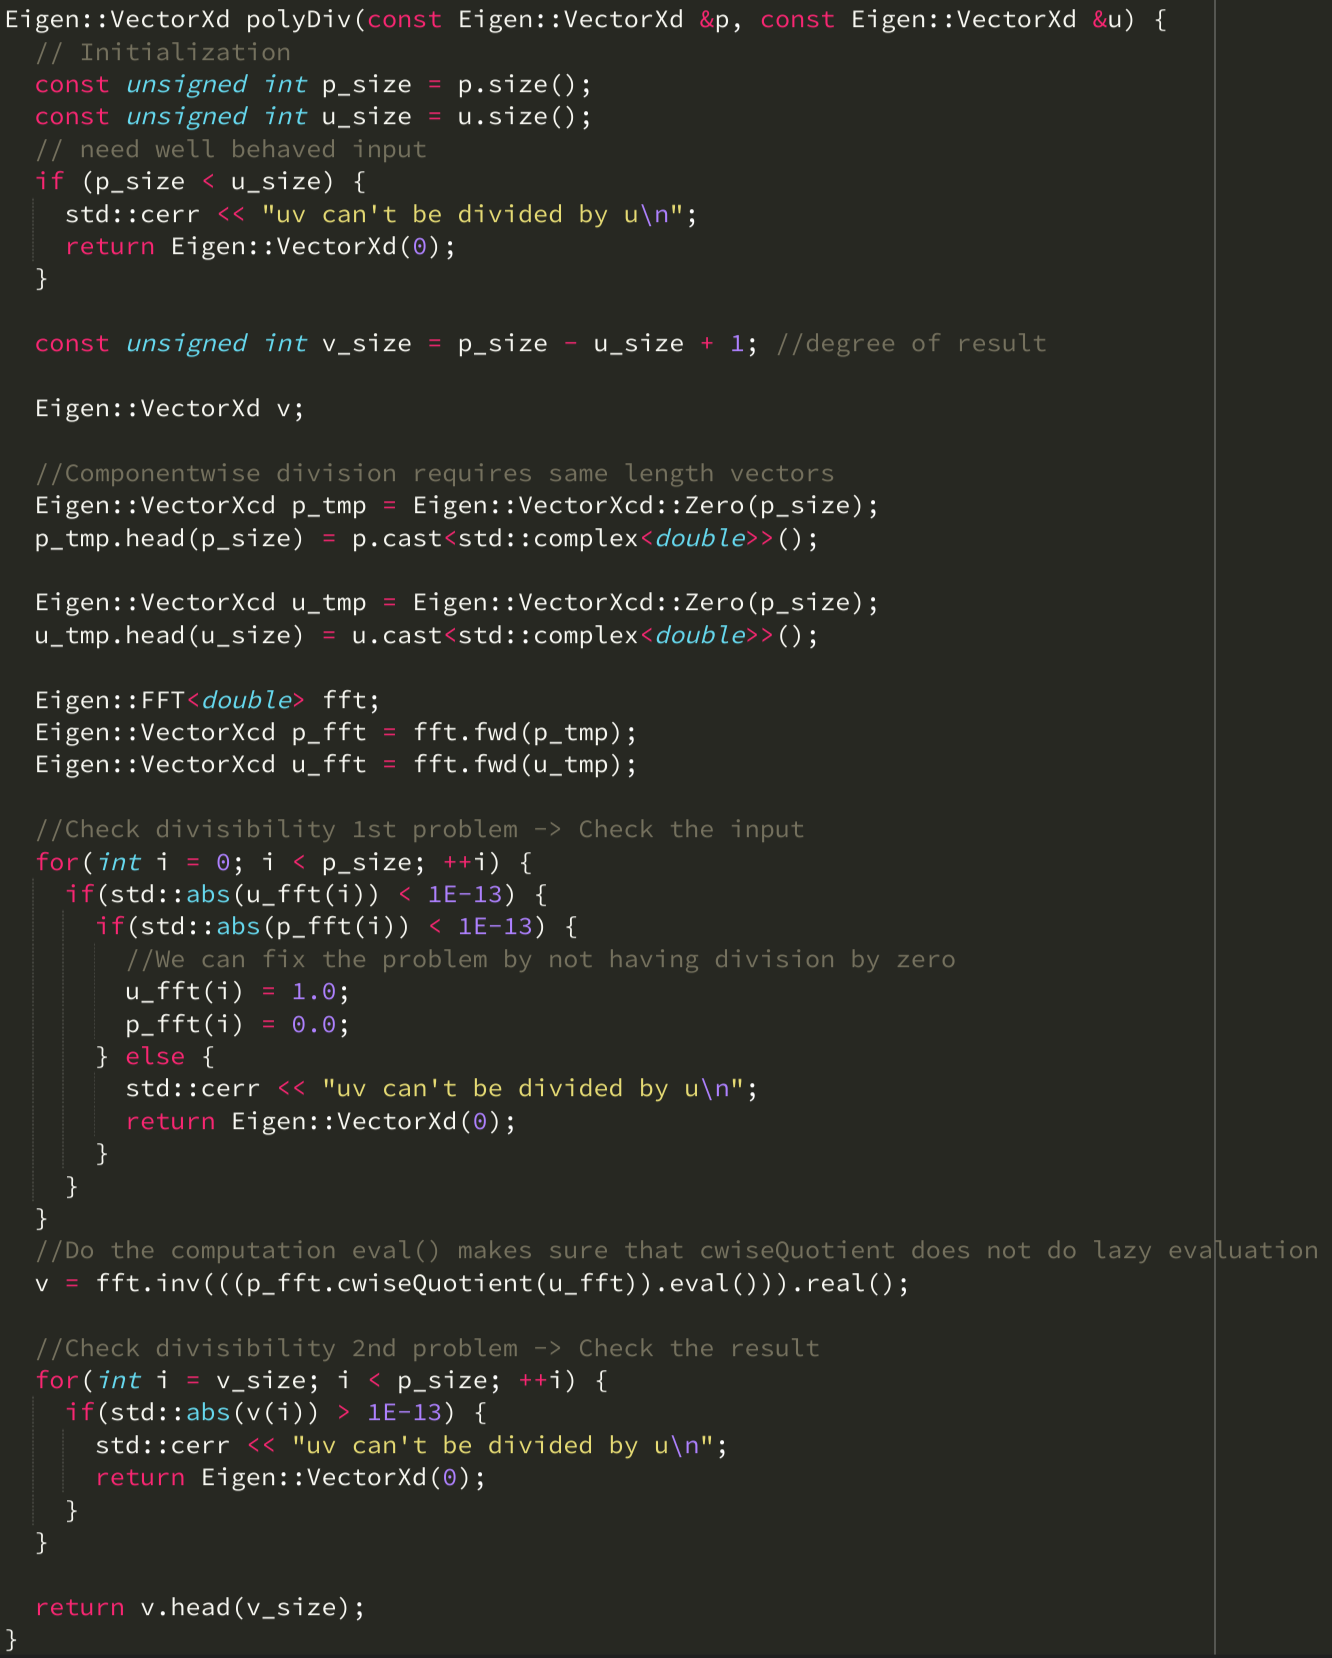
\includegraphics[width=1.0\linewidth]{4-3.d.png}
\end{figure}

\end{document}
